% The MIT License (MIT)
%
% Copyright (c) 2020 Yegor Bugayenko
%
% Permission is hereby granted, free of charge, to any person obtaining a copy
% of this software and associated documentation files (the "Software"), to deal
% in the Software without restriction, including without limitation the rights
% to use, copy, modify, merge, publish, distribute, sublicense, and/or sell
% copies of the Software, and to permit persons to whom the Software is
% furnished to do so, subject to the following conditions:
%
% The above copyright notice and this permission notice shall be included
% in all copies or substantial portions of the Software.
%
% THE SOFTWARE IS PROVIDED "AS IS", WITHOUT WARRANTY OF ANY KIND, EXPRESS OR
% IMPLIED, INCLUDING BUT NOT LIMITED TO THE WARRANTIES OF MERCHANTABILITY,
% FITNESS FOR A PARTICULAR PURPOSE AND NON-INFRINGEMENT. IN NO EVENT SHALL THE
% AUTHORS OR COPYRIGHT HOLDERS BE LIABLE FOR ANY CLAIM, DAMAGES OR OTHER
% LIABILITY, WHETHER IN AN ACTION OF CONTRACT, TORT OR OTHERWISE, ARISING FROM,
% OUT OF OR IN CONNECTION WITH THE SOFTWARE OR THE USE OR OTHER DEALINGS IN THE
% SOFTWARE.

% \documentclass[a4paper,UKenglish,cleveref, autoref]{lipics-v2019}
\documentclass[12pt]{article}
\title{What Happens to Constructors When Classes Get Larger?}
\author{Yegor Bugayenko}{}{}
% \authorrunning{Yegor Bugayenko}
% \ccsdesc[100]{Software and its engineering~Object oriented languages}
% \keywords{Object-Oriented Programming, Immutability, NCSS}
\usepackage[utf8]{inputenc}
\usepackage[numbers]{natbib}
\bibliographystyle{plainnat}
\usepackage[inline]{enumitem}
\usepackage{amsmath}
\usepackage{graphicx}
\usepackage{pgfplots}
\usepackage{verbatimbox}
\usepackage{interval}
\usepackage{hyperref}
\usepackage{minted}
  \setminted{fontsize=\footnotesize}
  \setminted{breaklines}
  \usemintedstyle{bw}
\newcommand{\code}[1]{\texttt{#1}}
\newenvironment{nicetable}
  {\setlength{\parindent}{0em}\medskip\small}
  {\medskip}
\def\thetotaljavafiles{10023}
\def\thetotalrepos{240}

\begin{document}
\raggedbottom
\maketitle

\begin{abstract}
...
\end{abstract}

\section{Introduction}


\section{Related Work}

...

\section{Empirical Results}

A list of Java repositories were retrieved from GitHub via their
public API. The first \thetotalrepos{} repositories were taken, which satisfied
the selection criteria:
\begin{enumerate*}[label={\arabic*)}]
\item more than 1,000 GitHub stars,
\item more than 200 Kb of data,
\item not archived, and
\item public.
\end{enumerate*}
The list included popular Java open source products, such as
Spring, RxJava, Guava, MyBatis, Clojure, JUnit, Lombok,
Graal, Selenium, Spark, Mockito, Neo4j, Jenkins, Netty, and others.

Files with \texttt{.java} extension were taken from all repositories.
Enums and interfaces were removed.
There were \thetotaljavafiles{} files found.

Attributes and constructors were counted for each Java class,
using \texttt{javalang}, an open source Java-parsing library written in Python.
The size of each class was calculated using the NCSS metric.
Classes with NCSS larger than 1000 were excluded from the graph. This decision was
motivated by the confounding effect the size of a class has
on the validity of object-oriented metrics, as was empirically shown by~\citet{el2001}.

The Figure~\ref{fig:1} demonstrates the relationship between NCSS (the horizontal
axis) and the amount of constructors in each class (the vertical axis). The
graph visually confirms the obvious thought: when classes get larger
they tend to have more constructors.

\begin{figure}[h]
  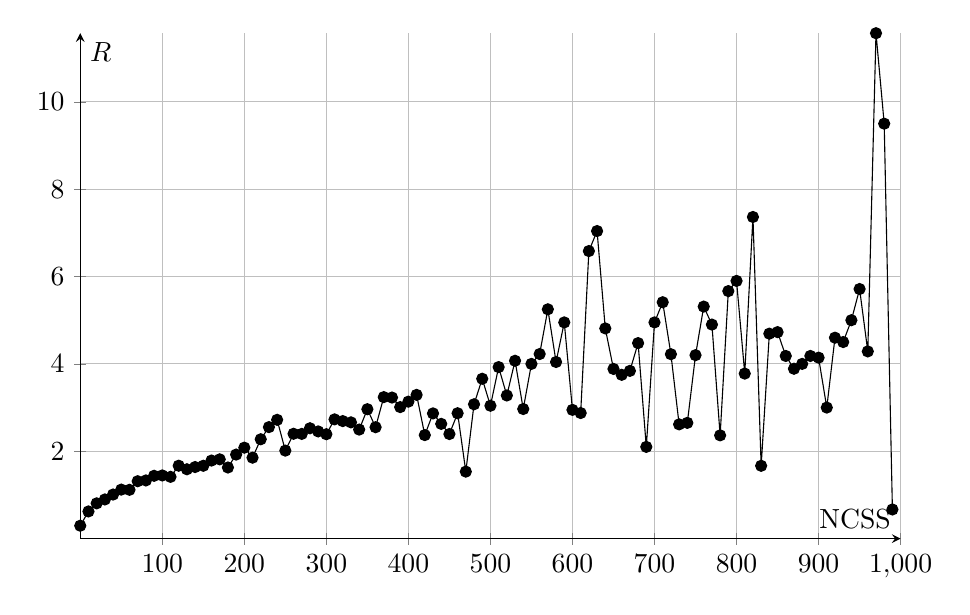
\begin{tikzpicture}
\begin{axis}[width=12cm,height=8cm,
axis lines=middle, xlabel={NCSS}, ylabel={$R$},
xmin=0, xmax=1000, ymin=0, ymax=11.571428571428571,
extra tick style={major grid style=black},grid=major]
\addplot [mark=*] coordinates {
(0,0.2949629574476006)
(10,0.621972219033406)
(20,0.8068989426243717)
(30,0.8960925833748133)
(40,1.008630902013877)
(50,1.1217015468607825)
(60,1.117018117018117)
(70,1.3134666163711808)
(80,1.3315460232350314)
(90,1.4375340971085653)
(100,1.445910290237467)
(110,1.4136858475894245)
(120,1.6690582959641256)
(130,1.5873836608066183)
(140,1.6382428940568476)
(150,1.6676096181046676)
(160,1.7868284228769498)
(170,1.8149405772495755)
(180,1.6276150627615062)
(190,1.9236276849642004)
(200,2.0819277108433734)
(210,1.853018372703412)
(220,2.2745098039215685)
(230,2.5526315789473686)
(240,2.7193548387096773)
(250,2.014423076923077)
(260,2.4)
(270,2.3969072164948453)
(280,2.526570048309179)
(290,2.454081632653061)
(300,2.389830508474576)
(310,2.72992700729927)
(320,2.6904761904761907)
(330,2.6611570247933884)
(340,2.4960629921259843)
(350,2.962962962962963)
(360,2.55)
(370,3.2395833333333335)
(380,3.229357798165138)
(390,3.010752688172043)
(400,3.1358024691358026)
(410,3.2906976744186047)
(420,2.3698630136986303)
(430,2.8666666666666667)
(440,2.6266666666666665)
(450,2.393939393939394)
(460,2.8703703703703702)
(470,1.5333333333333334)
(480,3.0754716981132075)
(490,3.6595744680851063)
(500,3.0416666666666665)
(510,3.926829268292683)
(520,3.276595744680851)
(530,4.071428571428571)
(540,2.966666666666667)
(550,4.0)
(560,4.225806451612903)
(570,5.25)
(580,4.043478260869565)
(590,4.95)
(600,2.9473684210526314)
(610,2.875)
(620,6.583333333333333)
(630,7.041666666666667)
(640,4.8125)
(650,3.8846153846153846)
(660,3.75)
(670,3.84)
(680,4.476190476190476)
(690,2.1)
(700,4.95)
(710,5.411764705882353)
(720,4.222222222222222)
(730,2.6153846153846154)
(740,2.65)
(750,4.2)
(760,5.3125)
(770,4.9)
(780,2.3636363636363638)
(790,5.666666666666667)
(800,5.9)
(810,3.7777777777777777)
(820,7.363636363636363)
(830,1.6666666666666667)
(840,4.6923076923076925)
(850,4.7272727272727275)
(860,4.181818181818182)
(870,3.888888888888889)
(880,4.0)
(890,4.181818181818182)
(900,4.142857142857143)
(910,3.0)
(920,4.6)
(930,4.5)
(940,5.0)
(950,5.714285714285714)
(960,4.285714285714286)
(970,11.571428571428571)
(980,9.5)
(990,0.6666666666666666)
};
\end{axis}\end{tikzpicture}

  \caption{The relationship between class size and the number of constructors}
  \label{fig:1}
\end{figure}

However, the Figure~\ref{fig:2} shows what happens at the same time
with the constructors-to-methods ratio. In smaller classes constructors
constitute 15-20\% of all methods, while for larger classes this ratio
drops below 10\%.

\begin{figure}[h]
  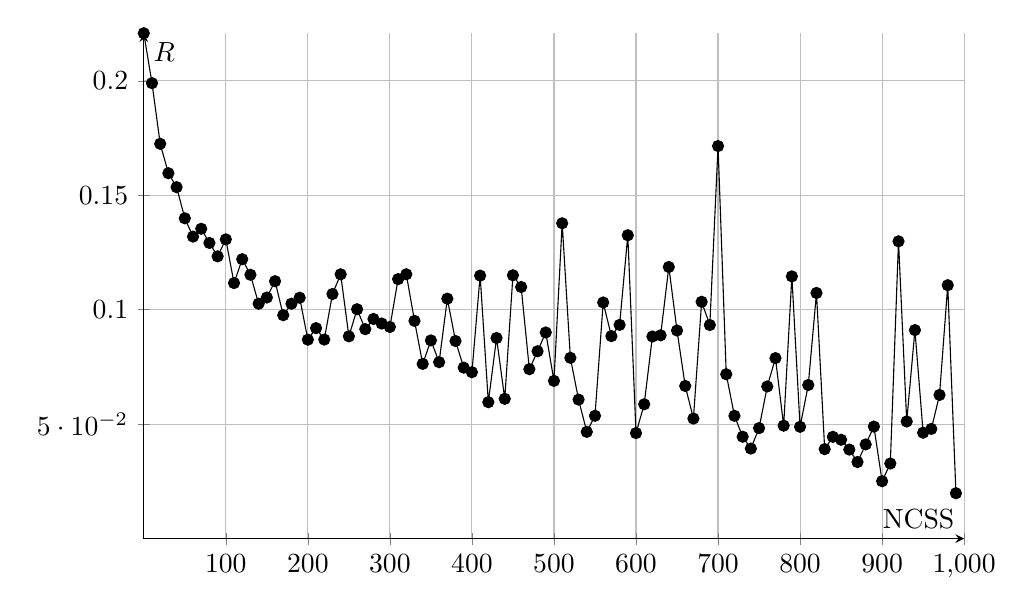
\begin{tikzpicture}
\begin{axis}[width=12cm,height=8cm,
axis lines=middle, xlabel={NCSS}, ylabel={$R$},
xmin=0, xmax=1000, ymin=0, ymax=0.22082909390897854,
extra tick style={major grid style=black},grid=major]
\addplot [mark=*] coordinates {
(0,0.22082909390897854)
(10,0.19900694958016843)
(20,0.1724960052893887)
(30,0.15965273219856857)
(40,0.1535575554780779)
(50,0.13994997763904912)
(60,0.13195071495615657)
(70,0.13536770556386907)
(80,0.12918033912575883)
(90,0.12332042007583346)
(100,0.13074664536864528)
(110,0.11166357520495679)
(120,0.12207768349773544)
(130,0.11526974377771763)
(140,0.10263225882162295)
(150,0.10533635199474517)
(160,0.1124701969451122)
(170,0.09761819314557124)
(180,0.10263832804519891)
(190,0.10524040275341504)
(200,0.0869154894305119)
(210,0.09196219792823211)
(220,0.08695371035859857)
(230,0.10685500455524288)
(240,0.11548016660063747)
(250,0.08838678917299685)
(260,0.10021678157824282)
(270,0.09151429354787813)
(280,0.09596654929401817)
(290,0.0939712918063595)
(300,0.09247884881327938)
(310,0.11337677988459384)
(320,0.11549494678253189)
(330,0.09514032272569009)
(340,0.07634161188769982)
(350,0.08660205165685209)
(360,0.07708846576877881)
(370,0.10483526280668586)
(380,0.08633103572783547)
(390,0.0746977009651164)
(400,0.0726996640095446)
(410,0.1149083508305553)
(420,0.05960354074501879)
(430,0.08764673584567836)
(440,0.06107470390662186)
(450,0.1150584286746777)
(460,0.10993853825909006)
(470,0.07402747219047028)
(480,0.08186608525192617)
(490,0.09006733378255374)
(500,0.0689162402243258)
(510,0.13777415766206774)
(520,0.07897527315706857)
(530,0.06073268590106369)
(540,0.04663807379072208)
(550,0.053663121214937194)
(560,0.10317177622969007)
(570,0.08846936554207757)
(580,0.09337237945752946)
(590,0.132550531578122)
(600,0.046104536591185644)
(610,0.05868970418211465)
(620,0.08830457611515509)
(630,0.08882526925412336)
(640,0.11868232534257923)
(650,0.09092161094190986)
(660,0.06669292561974703)
(670,0.05245423684564031)
(680,0.1034638298420516)
(690,0.09332242038088721)
(700,0.17152474478204818)
(710,0.07180754082214526)
(720,0.0536490689497568)
(730,0.04451096260174068)
(740,0.03933463041676892)
(750,0.048268487383739796)
(760,0.06647817847893561)
(770,0.07886306373926745)
(780,0.04933073348548323)
(790,0.11457431457431458)
(800,0.04884408257471778)
(810,0.0671117988537441)
(820,0.10733074271418258)
(830,0.0390909625481349)
(840,0.04446659252841066)
(850,0.043184467314623276)
(860,0.038902254100052)
(870,0.03344859386992238)
(880,0.041150637440108065)
(890,0.0489416436658803)
(900,0.02507128441677703)
(910,0.03281221922731357)
(920,0.12989616899391335)
(930,0.051182327477152435)
(940,0.09111086458312592)
(950,0.04627825753664681)
(960,0.04792581771876898)
(970,0.0627747117160798)
(980,0.11072310817959949)
(990,0.01982250908238246)
};
\end{axis}\end{tikzpicture}

  \caption{The relationship between class size and the constructors-to-methods ratio}
  \label{fig:2}
\end{figure}

This confirms that...

\section{Conclusion}

It was empirically confirmed that ...

The source code of Ruby and Python scripts used to do the research
is available in GitHub repository \texttt{yegor256/ctors-vs-size}.

\bibliography{main}

\end{document}
